\documentclass[11pt]{article}
\usepackage{graphicx}
\usepackage{amsmath,amsthm,amsfonts}
\usepackage{epsfig,graphics}
\usepackage{hyperref}
\usepackage{verbatim}
\usepackage{mathrsfs}
\usepackage{xcolor}

\setlength{\textheight}{8.5in}
\setlength{\evensidemargin}{0.0in}
\setlength{\oddsidemargin}{0.0in}
\setlength{\topmargin}{-0.5in}
\setlength{\textwidth}{6.5in}

\newtheorem{theorem}{Theorem}
\newtheorem*{theorem*}{Theorem}
\newtheorem{claim}{Claim}
\newtheorem*{claim*}{Claim}
\newtheorem{lemma}{Lemma}
\newtheorem*{lemma*}{Lemma}
\newtheorem{exercise}{Exercise}
\newtheorem*{exercise*}{Exercise}
\newtheorem{corollary}{Corollary}
\theoremstyle{definition}
\newtheorem{definition}{Definition}
\newtheorem{fact}{Fact}
\newtheorem*{fact*}{Fact}



\newcommand{\handout}[6]{
   \renewcommand{\thepage}{#1-\arabic{page}}
   \noindent
   \begin{center}
      \vbox{
    \hbox to \textwidth { #2 \hfill #3 }
       \vspace{4mm}
       \hbox to \textwidth { {\Large \hfill #4  \hfill} }
       \vspace{2mm}
       \hbox to \textwidth { { #5 \hfill #6} }
      }
   \hrulefill
   \end{center}
   \vspace*{4mm}
}

%\newcommand{\lecture}[5]{\handout{#1}{#2}{#3}{#4}{#5}}


% Types of Variables
\newcommand{\bvar}[1]{\mathbf{#1}} % bold variable
\newcommand{\mvar}[1]{\bvar{#1}} % matrix variable
\newcommand{\vvar}[1]{\vec{#1}} % vector variable

% Domains
\newcommand{\R}{\mathbb{R}}
\newcommand{\Z}{\mathbb{Z}}
\newcommand{\redgevec}{\R^{E}}
\newcommand{\rvertvec}{\R^{V}}
\newcommand{\rPos}{\R^{+}}
\newcommand{\rNonNeg}{\R^{\geq 0}}

% Symbol for definitions
\newcommand{\defeq}{\stackrel{\mathrm{\scriptscriptstyle def}}{=}}

% Optimization
\DeclareMathOperator*{\argmin}{arg\,min}
\DeclareMathOperator{\Cone}{Cone}
\DeclareMathOperator{\Cut}{CUT}

% Types of Graphs
\newcommand{\nlap}{\mathscr{L}_G}
\newcommand{\pseudo}[1]{{#1}^\dagger}
\newcommand{\lapPseudo}{\pseudo{\lap}}
\newcommand{\adj}{A}
\newcommand{\incMatrix}{\mvar{B}}
\newcommand{\diag}{\operatorname{diag}}
\newcommand{\rMatrix}{\mvar{R}} % resistance matrix
\newcommand{\iMatrix}{\mvar{I}} % identity matrix
\newcommand{\Vol}{\textrm{Vol}}


% Vectors
\newcommand{\1}{\vec{1}}
\renewcommand{\dot}[1]{\langle {#1} \rangle}

%other
\DeclareMathOperator{\sgn}{sgn}


\usepackage[symbol]{footmisc}
\usepackage{color}
\renewcommand{\thefootnote}{\fnsymbol{footnote}}
\setlength\parindent{0pt}
\begin{document}

\handout{}{CS 591 O1: Iterative Methods for Graph Algorithms and Network Analysis}{Fall 2018}{Lecture 6: Intro to Graph and Matrix Sparsification }{Instructor: Lorenzo Orecchia}{Scribe: Erasmo Tani}

\section*{A simple bound on $L$}

\begin{lemma}
For any graph $G$:
\[
    0 \preceq L_G \preceq 2D
\]
\end{lemma}
\begin{proof}
we have:
\[
    x^TL_Gx = \sum_{\{i,j\}\in E} (x_i - x_j)^2 \leq \sum_{\{i,j\}\in E} 2(x_i^2 + x_j^2) = 2 \sum_{i \in V}d_i x_i^2 = 2x^TDx
\]
\end{proof}
\begin{lemma}
If $\exists x \neq 0: x^TL_Gx = 2x^TDx$
\end{lemma}

\begin{lemma}[From last time]
$\lambda_2 = 0 \iff G$ is disconnected.
\end{lemma}

\begin{lemma}
$\lambda_n(\mathcal{L}) = 2 \iff G$ is bipartite.
\end{lemma}

There are robust versions of both the above lemmas and we will see them in future classes.

\section*{Sparsification}
Given a graph $G=(V,E)$ then:
\[
    L_G = \sum_{e\in E} \chi_e\chi_e^T
\]
where:
\[
    \chi_{u,v}:= e_u - e_v
\]
note that the sign doesn't matter in general. Our goal is to construct a weighted graph $H=(V,E_H,w_h)$ s.t. ($\varepsilon$-sparsifier)
\begin{enumerate}
    \item $|| L_G- L_H||\leq \varepsilon$
    \item $H$ is sparse i.e. $|E_H|$ is small $\tilde{O}(n) = O(n\text{ polylog }n)$. 
\end{enumerate}


There are two different notions of error we are going to discuss:
\begin{description}
\item[Aboslute Error] Here we want:
\[|x^TL_Gx - x^TL_Hx| \leq \varepsilon \cdot x^TDx\]
This is an easy definition to work with however in some cases it does not represent our notion of similarity in a combinatorial sense. Consider the example given in Figure 1.
\begin{figure}[h]
    \centering
    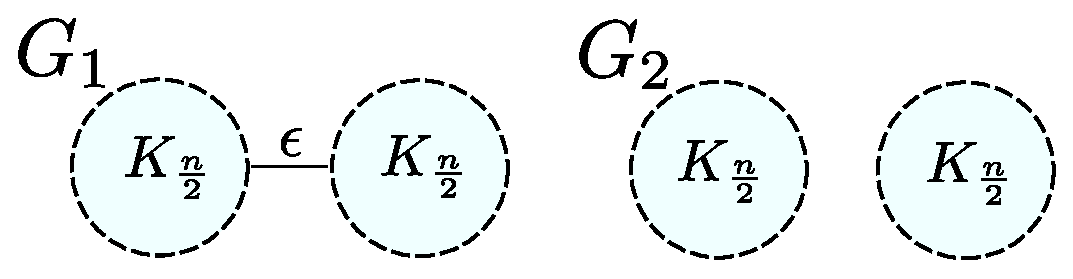
\includegraphics[scale=0.85]{additive-approximation-graphs.eps}
    \caption{Two graphs that are $\epsilon$-similar in additive error. Here $G_1$ is connected while $G_2$ is not.}
    \label{fig:my_label}
\end{figure}
In some sense  in this setting we are getting the small eigenvalues wrong.
\item[Relative Error]Here the measure of error is:
\[
    |x^TL_Gx - x^TL_Hx| \leq \varepsilon \cdot x^TL_Gx
\]
\end{description}

One thing worth nothing is that sparsifiers will approximately preserve the degree of every vertex (check by picking $x$ to be the indicator random vector of a vertex).
This holds independently of which of the two above notions of error is used. All the sparsifier we will look at have the additional property that $E_H \subseteq E_G$.

\section*{PSD Sparsification}
We are given a symmetric matrix $A \succeq 0$, $A \in \R^{n \times n}$ and it is given as the sum of rank 1 matrices:
\[
    A = \sum_{i=1}^m u_iu_i^T \hspace{2cm} m >>n
\]

$A$ is telling me how the mass of the $u_i$ vectors is distributed. Look for instance at:
\[
    x^TAx = \sum_{i=1}^n (u_i^Tx)^2
\]

we may want to construct a matrix sparsifier:
\[
    \tilde{A} = \sum_{i=1}^m s_i u_iu_i^T
\]
where we want:
\[
    \mathbb{E}[s_i]=1
\]

Choosing the distribution of the $s_i$s amounts to deciding the relative importance of each vector in the decomposition of $A$. (Statistical Leverage).

\[
    \forall x: \hspace{1cm} |x^TAx - x^T\tilde{A}x| \leq \varepsilon \cdot x^TAx
\]
we do a change of matrix: $y = A^{1/2}x$
\[
    |y^TIy - y^TA^{-1/2}\tilde{A} A^{-1/2}y| \leq \varepsilon \cdot ||y||^2
\]

\[
    \tilde{A} = \sum_{i=1}^T s_i A^{-1/2}u_iu_i^TA^{-1/2}
\]

Suppose you have a bunch of vectors $\{\vec{a}_i\}$ and you want to estimate the sum by sampling.
\[
    A =\sum_{i=1}^ma_i \hspace{2cm} \vec{a}_i \in \R^n, ||\vec{a}_i||^2
\]
 we can do:
 \[
    s_i = \begin{cases} \frac{1}{p_i} & \text{w.p. } \,p_i \propto ||a_i||^2\\
    0 
    \end{cases}
 \]
\section*{Matrix Chernoff Bounds}
 \subsection*{Scalar Chernoff Bound} Given a sum of independent random variabels:
 \[
    X = \sum X_i
 \]
 we can look at:
 \[
    g(\theta) = \mathbb{E}[e^{\theta X}] = \mathbb{E}[e^{\theta \Sigma X_i}] = \prod \mathbb{E}[e^{\theta X_i}]
 \]
 We then have:
 \[
    Pr[X > \lambda ] = Pr[e^{\theta X} > e^{\theta\lambda}] \leq \frac{\mathbb{E}[e^{\theta x}]}{e^{\theta \lambda}}
 \]
 \subsection*{Matrix Chernoff Bound}
 Given a matrix random variable $Y \in S^{n \times n}$ its mgf is:
 \[
    \mathbb{E}[e^{\theta Y}]
 \]
 where $e^{\theta Y}$ is a matrix exponential.
\end{document}
